\documentclass[11pt,a4paper]{article}
\usepackage[margin=2.3cm]{geometry}
\usepackage[T1]{fontenc}
\usepackage{textcomp}
\input{glyphtounicode}
\pdfgentounicode=1
\usepackage{lmodern}
\usepackage{xcolor}
\usepackage{listings}
\usepackage{tcolorbox}
\usepackage{booktabs}
\usepackage{array}
\usepackage{tikz}
\usepackage{hyperref}
\hypersetup{colorlinks=true, linkcolor=blue!50!black, citecolor=green!40!black}

\definecolor{codebg}{RGB}{248,248,245}
\lstset{
  language=C, basicstyle=\ttfamily\footnotesize, backgroundcolor=\color{codebg},
  keywordstyle=\color{blue!60!black}\bfseries, commentstyle=\color{green!45!black}\itshape,
  stringstyle=\color{red!60!black}, numbers=none, upquote=true,
  frame=single, rulecolor=\color{gray!40}, breaklines=true, columns=fullflexible,
  keepspaces=true, showstringspaces=false, morekeywords={omp_lock_t}
}
\lstdefinestyle{sh}{language=bash, backgroundcolor=\color{black!5}}

\newtcolorbox{keyidea}{colback=blue!4, colframe=blue!45!black, title=Key ideas, fonttitle=\bfseries\small}
\newtcolorbox{experiment}{colback=orange!5, colframe=orange!70!black, title=Experiment, fonttitle=\bfseries\small}

\title{\textbf{OpenMP --- Lesson 9}\\[4pt]\large Locks}
\author{Gustavo Lozano}
\date{November 2026}

\begin{document}
\maketitle

\noindent\textit{\small Source: Chapman, Jost \& van der Pas~\cite{chapman}, Ch.~4
``OpenMP Language Features'' (the lock routines of the runtime library).}

\section{The idea}
In Lesson~3, \texttt{critical} made an update safe by letting only one thread at a time
into a block. But \texttt{critical} is \textbf{one lock for the whole block}: two threads
that update \emph{different} data still wait for each other.

Example: a histogram. Thread~0 adds to bin 17, thread~1 adds to bin 512. There is no
conflict, yet with \texttt{critical} one of them waits. A \textbf{lock} is a variable you
create yourself, so you can have \textbf{one lock per bin}. Threads then wait only when they
really touch the same bin.

\begin{center}
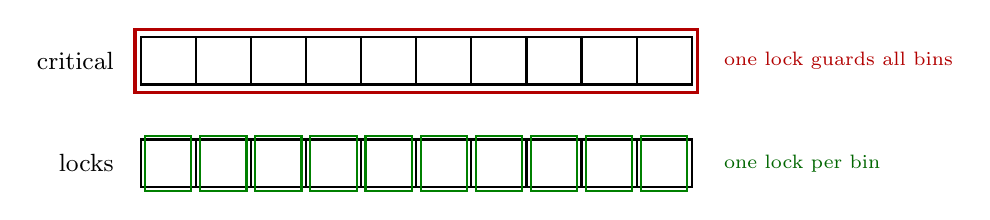
\begin{tikzpicture}[thick, x=0.7cm]
  \node[font=\small, anchor=east] at (-0.3,0.3) {critical};
  \foreach \i in {0,...,9} \node[draw, minimum width=0.7cm, minimum height=0.6cm, font=\tiny] at (\i+0.5,0.3) {};
  \draw[red!70!black, very thick] (-0.1,-0.1) rectangle (10.1,0.7);
  \node[font=\scriptsize, red!70!black, anchor=west] at (10.4,0.3) {one lock guards all bins};
  \node[font=\small, anchor=east] at (-0.3,-1.0) {locks};
  \foreach \i in {0,...,9} {
    \node[draw, minimum width=0.7cm, minimum height=0.6cm, font=\tiny] at (\i+0.5,-1.0) {};
    \draw[green!50!black] (\i+0.08,-1.35) rectangle (\i+0.92,-0.65);
  }
  \node[font=\scriptsize, green!40!black, anchor=west] at (10.4,-1.0) {one lock per bin};
\end{tikzpicture}
\end{center}

\section{The lock routines}
A lock has type \texttt{omp\_lock\_t} and a fixed life cycle:
\begin{center}
\small
\begin{tabular}{@{}>{\raggedright\arraybackslash}p{4.6cm}>{\raggedright\arraybackslash}p{10.6cm}@{}}
\toprule
Routine & Meaning \\ \midrule
\texttt{omp\_init\_lock(\&l)} & create the lock (unlocked); before any use \\
\texttt{omp\_set\_lock(\&l)} & acquire it; if another thread holds it, \textbf{wait} \\
\texttt{omp\_unset\_lock(\&l)} & release it; one waiting thread may now acquire it \\
\texttt{omp\_destroy\_lock(\&l)} & free it; after the last use \\
\bottomrule
\end{tabular}
\end{center}
The danger: if a thread forgets \texttt{omp\_unset\_lock} (for example, because of an early
\texttt{return} or \texttt{break}), every other thread that wants that lock waits forever.
The program \textbf{hangs} (a \emph{deadlock}). \texttt{critical} cannot be forgotten
this way, which is why it is preferred when one lock is enough.

\section{The code}
\lstinputlisting[title=\texttt{locks.c}]{locks.c}

\begin{lstlisting}[style=sh]
gcc -Wall -fopenmp -o locks locks.c
OMP_NUM_THREADS=2 ./locks
\end{lstlisting}
Output on a 2-core machine (your times will differ):
\begin{lstlisting}[style=sh]
critical      : 2.332 s   total = 20000000
lock per bin  : 0.481 s   total = 20000000
\end{lstlisting}

\begin{keyidea}
\begin{itemize}
  \item Both histograms are correct (\texttt{total = N}). They differ only in how long
        threads wait.
  \item With one lock per bin, threads wait only when they hit the same bin at the same
        moment, which is rare with 1000 bins.
  \item Every \texttt{omp\_set\_lock} is matched by an \texttt{omp\_unset\_lock} on the
        same lock, a few lines later, with nothing in between that could skip it.
\end{itemize}
\end{keyidea}

\section{The experiment}
\begin{experiment}
\textbf{Question:} when does a lock per data item beat one global lock?
\begin{enumerate}
  \item Run with 1 thread and with \texttt{nproc} threads:
\begin{lstlisting}[style=sh]
OMP_NUM_THREADS=1 ./locks
OMP_NUM_THREADS=$(nproc) ./locks
\end{lstlisting}
  \item Change \texttt{\#define NBINS 1000} to \texttt{\#define NBINS 2}, recompile, and
        repeat step 1.
\end{enumerate}
\textbf{What to observe and answer.}
\begin{enumerate}
  \item With 1000 bins, why does \texttt{critical} get so much slower with more threads,
        while locks per bin suffer much less?
  \item With 2 bins, why do locks per bin lose most of their advantage?
  \item Even the lock version with several threads is slower than with 1 thread. Why,
        and what would be the real fix?
\end{enumerate}
\end{experiment}

\paragraph{Answers (read after trying).}
(1)~With \texttt{critical} every update needs the same lock, so all updates form a single
line, and the lock is handed from core to core on almost every iteration (on the 2-core
test machine: 0.26\,s with 1 thread, 2.33\,s with 2). With 1000 locks, two threads rarely
want the same one at the same moment (0.48\,s).
(2)~With 2 bins, half of the time both threads want the same bin, so they wait for each
other again, just as with \texttt{critical} (2.06\,s for locks vs.\ 3.19\,s for
\texttt{critical} on the test machine). A lock per item only helps when conflicts on the
same item are rare. This is called \emph{lock granularity}.
(3)~Each update still pays for acquiring and releasing a lock, and neighbouring bins and
locks share cache lines, so the threads also suffer false sharing (Lesson~8). Locks make
the update \emph{safe}, not \emph{fast}. The real fix is to avoid sharing: each thread
fills a \emph{private} histogram and they are added together once at the end. OpenMP can do
this for you with an array reduction, \texttt{reduction(+:hist[:NBINS])}, available since
OpenMP~4.5 (newer than the Chapman book; see van der Pas et al.~\cite{vdp}). On the test
machine this version takes 0.010\,s with 2 threads, against 0.48\,s with locks.

\paragraph{Next lesson.} Finding races with a tool: compiling with ThreadSanitizer and
reading its report on the buggy counter from Lesson~2 (Chapman et al., Ch.~7).

\begin{thebibliography}{9}
\bibitem{chapman} B.~Chapman, G.~Jost, and R.~van der Pas. \emph{Using OpenMP: Portable
  Shared Memory Parallel Programming}. MIT Press, Cambridge, MA, 2007.
\bibitem{vdp} R.~van der Pas, E.~Stotzer, and C.~Terboven. \emph{Using OpenMP --- The Next
  Step: Affinity, Accelerators, Tasking, and SIMD}. MIT Press, Cambridge, MA, 2017.
\end{thebibliography}
\end{document}
